%----------------------------------------------------------------------------------------
% METADATA BLOCK (YAML)  — see inbox/README.md
%----------------------------------------------------------------------------------------
% uid: ""
% school: "lycee"
% level: "2eme"
% section: ["Sciences", "Informatique"]
% chapter: "Barycentre"
% title: "Synthèse : barycentre partiel et droites concourantes"
% difficulty: "Moyen"
% tags: ["barycentre", "barycentre-partiel", "droites-concourantes"]
% provenance: "own"
% batch: "2026-11-19-2sc-polynomes-barycentre"
%----------------------------------------------------------------------------------------

\newcommand{\R}{\mathbb{R}}
\newcommand{\vect}[1]{\overrightarrow{#1}}

% ---STATEMENT---
Soit $ABC$ un triangle. On considère :
$I$ le barycentre de $(B,1)$ et $(C,2)$ ;\quad $J$ le barycentre de $(A,3)$ et $(C,2)$ ;\quad $K$ le barycentre de $(A,3)$ et $(B,1)$ ;\quad $G$ le barycentre de $(A,3)$, $(B,1)$ et $(C,2)$.
\begin{center}
% alt: Triangle ABC.
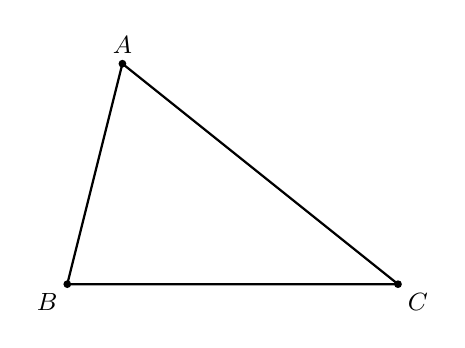
\begin{tikzpicture}[scale=0.7, font=\small]
  \coordinate (A) at (1,4); \coordinate (B) at (0,0); \coordinate (C) at (6,0);
  \draw[thick] (A)--(B)--(C)--cycle;
  \foreach \p/\pos in {A/above, B/below left, C/below right} \fill (\p) circle (2pt) node[\pos] {$\p$};
\end{tikzpicture}
\end{center}
\begin{enumerate}
  \item Exprimer $\vect{BI}$, $\vect{AJ}$ et $\vect{AK}$ à l'aide de $\vect{BC}$, $\vect{AC}$ et $\vect{AB}$, puis construire $I$, $J$ et $K$.
  \item Montrer que $G$ est le milieu du segment $[AI]$.
  \item Montrer que $G$ appartient aux droites $(BJ)$ et $(CK)$. Que peut-on dire des droites $(AI)$, $(BJ)$ et $(CK)$ ?
  \item Montrer que $\vect{AG}=\dfrac16\vect{AB}+\dfrac13\vect{AC}$.
\end{enumerate}

% ---SOLUTION---
\begin{center}
% alt: Triangle ABC avec I sur [BC], J sur [AC], K sur [AB] et les droites (AI), (BJ), (CK) concourantes en G.
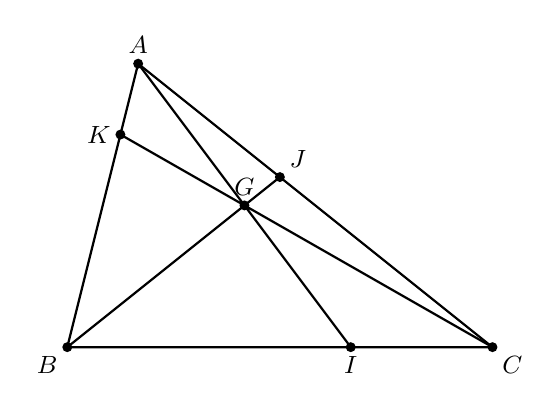
\begin{tikzpicture}[scale=0.9, font=\small]
  \coordinate (A) at (1,4); \coordinate (B) at (0,0); \coordinate (C) at (6,0);
  \coordinate (I) at (4,0); \coordinate (J) at (3,2.4); \coordinate (K) at (0.75,3); \coordinate (G) at (2.5,2);
  \draw[thick] (A)--(B)--(C)--cycle;
  \draw[thick] (A)--(I) (B)--(J) (C)--(K);
  \foreach \p/\pos in {A/above, B/below left, C/below right, I/below, J/above right, K/left, G/above}
    \fill (\p) circle (2pt) node[\pos] {$\p$};
\end{tikzpicture}
\end{center}
\begin{enumerate}[itemsep=14pt]
  \item
  \begin{prop}[Position du barycentre de deux points]
  Si $G$ est le barycentre de $(A,\alpha)$ et $(B,\beta)$, $\alpha+\beta\neq0$ : \ib{$\vect{AG}=\dfrac{\beta}{\alpha+\beta}\vect{AB}$}.
  \end{prop}
  \[\vect{BI}=\dfrac{2}{1+2}\vect{BC}=\dfrac23\vect{BC}\qquad\vect{AJ}=\dfrac{2}{3+2}\vect{AC}=\dfrac25\vect{AC}\qquad\vect{AK}=\dfrac{1}{3+1}\vect{AB}=\dfrac14\vect{AB}\]
  $I$ est aux deux tiers de $[BC]$ à partir de $B$, $J$ aux deux cinquièmes de $[AC]$ à partir de $A$, $K$ au quart de $[AB]$ à partir de $A$.

  \item
  \begin{prop}[Barycentre partiel]
  On peut remplacer deux des points par leur barycentre affecté de la \ib{somme de leurs coefficients}.
  \end{prop}
  On remplace $(B,1)$ et $(C,2)$ par $(I,3)$ : $G$ est le barycentre de $(A,3)$ et $(I,3)$.

  Les coefficients sont égaux : $G$ est le milieu de $[AI]$.

  \item On remplace $(A,3)$ et $(C,2)$ par $(J,5)$ : $G$ est le barycentre de $(B,1)$ et $(J,5)$, donc $G\in(BJ)$, avec $\vect{BG}=\dfrac56\vect{BJ}$.

  On remplace $(A,3)$ et $(B,1)$ par $(K,4)$ : $G$ est le barycentre de $(C,2)$ et $(K,4)$, donc $G\in(CK)$, avec $\vect{CG}=\dfrac46\vect{CK}=\dfrac23\vect{CK}$.

  \textbf{Conclusion :} les trois droites $(AI)$, $(BJ)$ et $(CK)$ sont \textbf{concourantes} en $G$.

  \item
  \begin{prop}[Relation vectorielle du barycentre]
  $G$ barycentre de $(A,\alpha)$, $(B,\beta)$, $(C,\gamma)$ : \ib{$\vect{AG}=\dfrac{\beta\vect{AB}+\gamma\vect{AC}}{\alpha+\beta+\gamma}$}.
  \end{prop}
  Ici $\alpha+\beta+\gamma=6$ :
  \[\vect{AG}=\dfrac{1\times\vect{AB}+2\times\vect{AC}}{6}=\dfrac16\vect{AB}+\dfrac13\vect{AC}\]
  \textbf{Contrôle} avec 2) : $\vect{AG}=\dfrac12\vect{AI}=\dfrac12\left(\vect{AB}+\dfrac23\vect{BC}\right)=\dfrac12\vect{AB}+\dfrac13\left(\vect{AC}-\vect{AB}\right)=\dfrac16\vect{AB}+\dfrac13\vect{AC}$ (vérifié)
\end{enumerate}
\textbf{Idée :} chaque droite joint un sommet au barycentre des deux autres points : l'associativité met $G$ sur les trois droites en même temps.

\textbf{Piège :} $G$ n'est pas le centre de gravité : les coefficients ne sont pas égaux, donc $G$ n'est pas aux deux tiers des droites.
